\newpage
\hypertarget{schema tex}{}
\subsection{Text Schema}
\texHeader

% Expand the crap outta all of this!

\begin{itemize}

\item[$\blacktriangleright$] Right-click on the \texttt{MyWorkingSet} folder, and navigate to ``New / TGG'' (Fig.~\ref{fig:contextTGG}).

\vspace{0.5cm}

\begin{figure}[htbp]
\begin{center}
  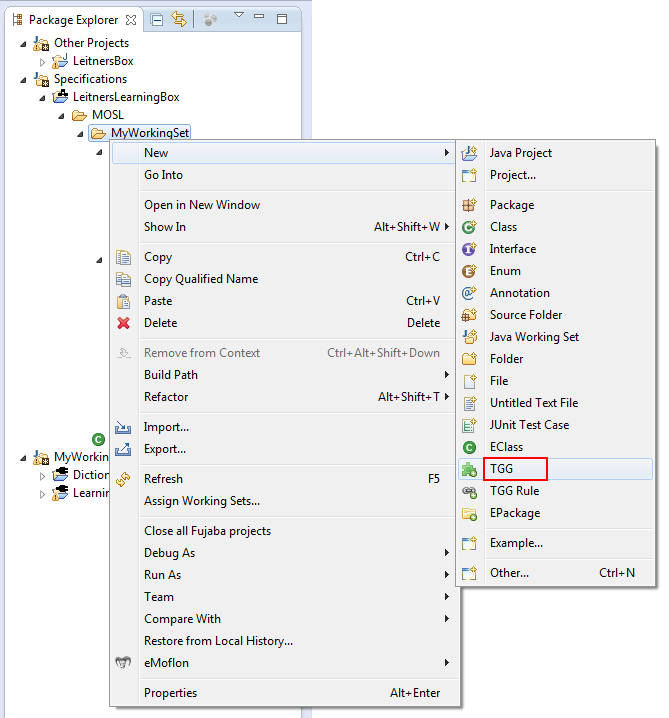
\includegraphics[width=0.8\textwidth]{eclipse_contextNewTGG}
  \caption{Creating a new TGG Schema}
  \label{fig:contextTGG}
\end{center}
\end{figure}

\item[$\blacktriangleright$] Name the TGG \texttt{LearningBoxToDictionaryIntegration}, setting the source as \texttt{LearningBoxLanguage} and target as
\texttt{DictionaryLanguage} (Fig.~\ref{fig:newTGG}).

\item[$\blacktriangleright$] A new \texttt{schema} file should now be active in the editor! This is the \emph{TGG Schema} which declares each
\emph{correspondence type} as an \texttt{integration class}. Press \texttt{ctrl + space bar} and use the auto completion to generate a new class template.

\newpage

\begin{figure}[htbp]
\begin{center}
  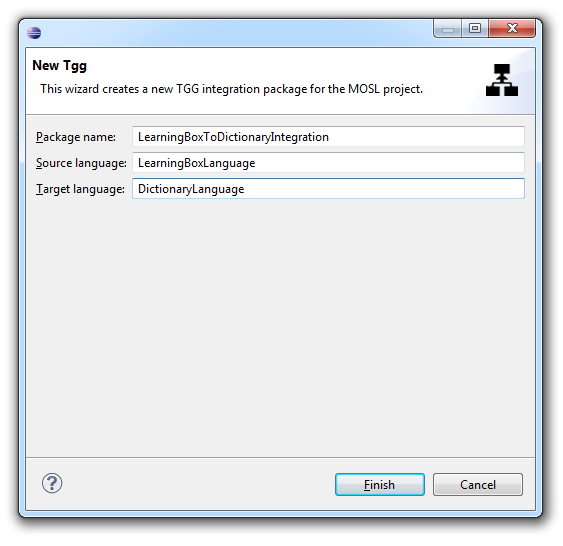
\includegraphics[width=0.8\textwidth]{eclipse_newTGG}
  \caption{Setting your \texttt{source} and \texttt{target} metamodels}
  \label{fig:newTGG}
\end{center}
\end{figure}

\item[$\blacktriangleright$] Note that you can press \texttt{tab} to quickly jump forward through each element. Name the class \texttt{BoxToDictionary}, and
list the source as \texttt{Box} and target as \texttt{Dictionary} (Fig.~\ref{fig:newTGG}). In the TGG Dialogue, you set the source and target \emph{classes}.
Here, you are creating the first object variables to represent them. 

\begin{figure}[htbp]
\begin{center}
  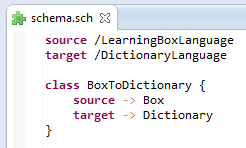
\includegraphics[width=0.4\textwidth]{eclipse_schemaFirstClass}
  \caption{Creating a correspondence type}
  \label{fig:firstCorrType}
\end{center}
\end{figure}

\item[$\blacktriangleright$] Believe it or not, that's all you need for your correspondence type! Your schema is now complete with connections to your
\texttt{source} and \texttt{target} metamodels via a \emph{link} metamodel. To see the equivalent structure in the visual syntax, check out
Fig.~\ref{fig:firstCorrType} from the previous section.

\end{itemize}
